% Author: Connor Baker
% Date Created: June 19, 2017
% Last Edited: June 19, 2017
% Version: 0.1a

% Declare type of document
\documentclass[10pt]{article}

% Import Packages
\usepackage[utf8]{inputenc}
\usepackage[mathscr]{euscript}
\usepackage{amsfonts,amsmath,amssymb,amsthm}
\usepackage{mathtools,mathdots}
\usepackage{enumitem}
\usepackage{array}
\usepackage{graphics}
\usepackage{longtable}
\usepackage{geometry}[left=0.5in,right=0.5in,top=0.5in,bottom=0.5in]
\usepackage{minted}
\usepackage{dirtytalk}
\usepackage{hyperref}
\hypersetup{colorlinks=true,urlcolor=blue}

% Define the basic math environments
\theoremstyle{definition}
\newtheorem{definition}[equation]{Definition}
\newtheorem{example}[equation]{Example}
\newtheorem{axiom}[equation]{Axiom}
\theoremstyle{plain}
\newtheorem{theorem}[equation]{Theorem}
\newtheorem{proposition}[equation]{Proposition}
\newtheorem{lemma}[equation]{Lemma}
\newtheorem{corollary}[equation]{Corollary}
\newtheorem{conjecture}[equation]{Conjecture}

% Define frequently used commands
\newcommand{\N}{\mathbb{N}}
\newcommand{\Z}{\mathbb{Z}}
\newcommand{\Q}{\mathbb{Q}}
\newcommand{\R}{\mathbb{R}}
\newcommand{\C}{\mathbb{C}}
\DeclareMathOperator\dom{dom}
\DeclareMathOperator\rang{rang}
\newcommand{\ds}{\displaystyle}

\makeatletter
\def\imod#1{\allowbreak\mkern10mu({\operator@font mod}\,\,#1)}
\makeatother

\begin{document} %This is where we type the text that we plan on having in our document.

% Create the Header
\begin{center}
  {\Large\textsc{Matrix Operations with AVX2 Instructions}}

  {\large Connor Baker, June 2017}
\end{center}
\section{Creating the Matrix}
Consider the following line of \texttt{C++}:
\begin{minted}[tabsize=2,breaklines]{c++}
std::vector<__m256> v(4, _mm256_setr_ps(0.0, 1.0, 2.0, 3.0, 4.0, 5.0, 6.0, 7.0));
\end{minted}
this statement creates a matrix (of sorts) named v, of four rows and eight columns, where each row is an Intel AVX2 (Advanced Vector Extensions 2) datatype.

\[
\text{v} =
\begin{bmatrix}
    0.0 & 1.0 & 2.0 & 3.0 & 4.0 & 5.0 & 6.0 & 7.0 \\
    0.0 & 1.0 & 2.0 & 3.0 & 4.0 & 5.0 & 6.0 & 7.0 \\
    0.0 & 1.0 & 2.0 & 3.0 & 4.0 & 5.0 & 6.0 & 7.0 \\
    0.0 & 1.0 & 2.0 & 3.0 & 4.0 & 5.0 & 6.0 & 7.0
\end{bmatrix}
\]

We can access any element of this matrix just like we would with a two dimensional array or vector, so the above corresponds to:

\[
\text{v} =
\begin{bmatrix}
    v[0][0] & v[0][1] & v[0][2] & v[0][3] & v[0][4] & v[0][5] & v[0][6] & v[0][7] \\
    v[1][0] & v[1][1] & v[1][2] & v[1][3] & v[1][4] & v[1][5] & v[1][6] & v[1][7] \\
    v[2][0] & v[2][1] & v[2][2] & v[2][3] & v[2][4] & v[2][5] & v[2][6] & v[2][7] \\
    v[3][0] & v[3][1] & v[3][2] & v[3][3] & v[3][4] & v[3][5] & v[3][6] & v[3][7]
\end{bmatrix}
\]

\noindent and as such, the elements are addressable. If we wanted to change every value of six to an 11, we can do so:
\begin{minted}{c++}
  for (size_t i = 0; i < 4; i++) {
    v[i][6] = 11.0;
  }
\end{minted}

\subsection{A Little More on AVX}
Intel's AVX has several datatypes of note (see next page), but for the purposes of this discussion, we will talk exclusively about the \texttt{\_\_m256} datatype, and its applications to matrix operations.

If you need an overview of how to use AVX, I highly recommend that you read Matt Scarpino's excellent article \href{https://www.codeproject.com/Articles/874396/Crunching-Numbers-with-AVX-and-AVX}{Crunching Numbers with AVX and AVX2} on Code Project.

\subsection{Why Use AVX?}
The benefit of using an Intel AVX2 data type is that we are then allowed to use intrinsic functions, which are essentially calls to highly optimized assembly instructions from within high-level languages. In doing this, we retain the readability and ease of use that makes high level langauges attractive, while being able to write highly-performant code in critical areas of programs.



\pagebreak



\vspace*{\fill}
\begin{figure}[h]
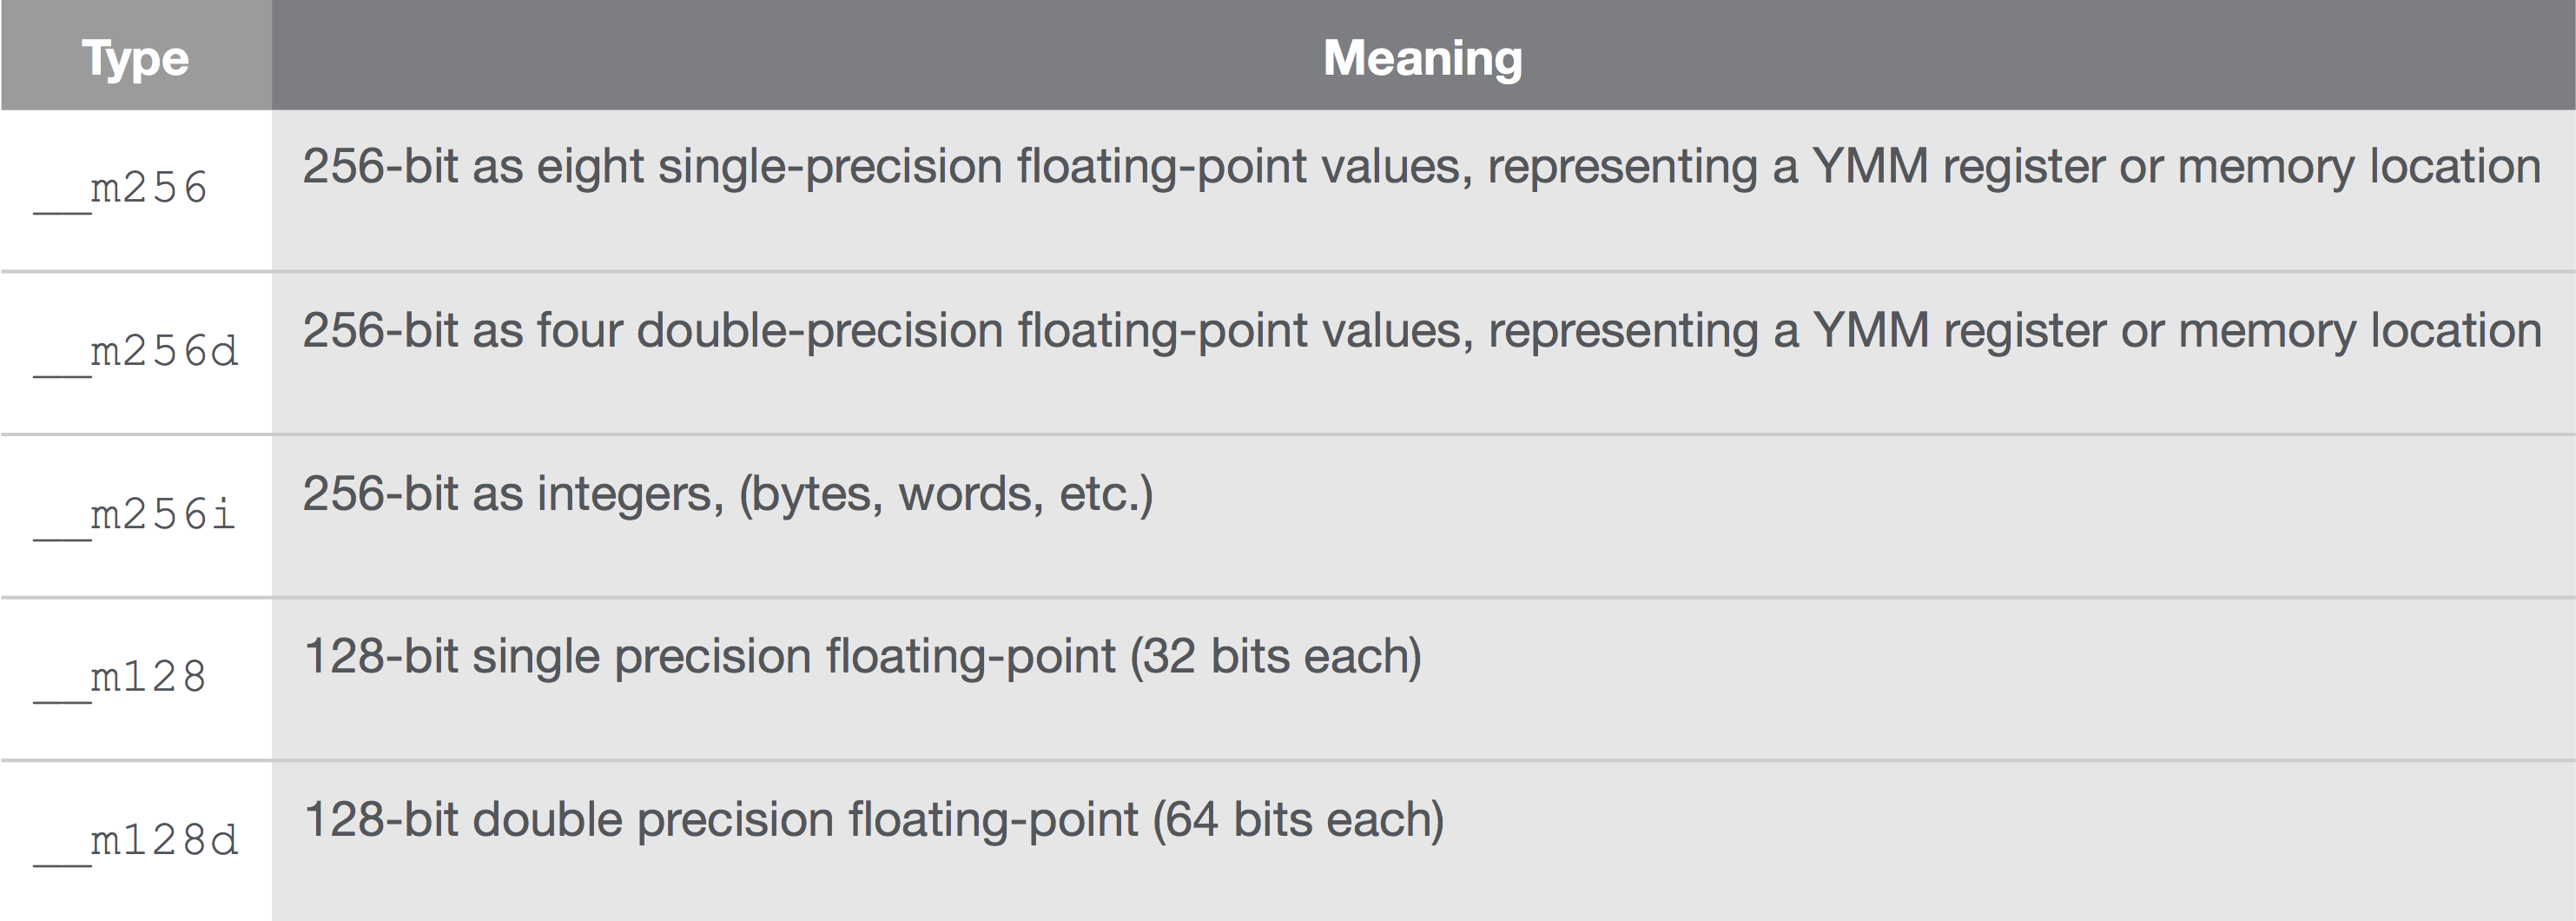
\includegraphics[width=\textwidth]{images/tbl1}
\caption{Intel AVX Data Types, retrived from \href{https://software.intel.com/en-us/articles/introduction-to-intel-advanced-vector-extensions}{Introduction to Intel® Advanced Vector Extensions}}
\centering
\end{figure}
\vspace*{\fill}



\pagebreak



\section{It's All About the Size (of the Row)}
Returning to our earlier code sample,
\begin{minted}[tabsize=2,breaklines]{c++}
std::vector<__m256> v(4, _mm256_setr_ps(0.0, 1.0, 2.0, 3.0, 4.0, 5.0, 6.0, 7.0));
\end{minted}
\noindent we see an issue in terms of the size of the matrix that we can generate. Our matrix is stuck at a size of $n\times 8$, since the AVX vector holds eight floats. But wait! Consider the following snippet:

\begin{minted}[tabsize=2,breaklines]{c++}
std::vector<std::vector<__m256>> v(SIZE, std::vector<__m256>(4, _mm256_setr_ps(1.0, 2.0, 3.0, 4.0, 5.0, 6.0, 7.0, 8.0)));

for (size_t i = 0; i < v.size(); i++) {
  for (size_t j = 0; j < v[0].size(); j++) {
      for (size_t k = 0; k < 8; k++) {
          std::cout << v[i][j][k] << ' ';
      }
      std::cout << '\t';
  }
  std::cout << std::endl;
}
\end{minted}
\noindent the output of which is below.

\begin{center}
  \begin{tabular}{c c c c}
    1 2 3 4 5 6 7 8 & 1 2 3 4 5 6 7 8 & 1 2 3 4 5 6 7 8 & 1 2 3 4 5 6 7 8 \\
    1 2 3 4 5 6 7 8 & 1 2 3 4 5 6 7 8 & 1 2 3 4 5 6 7 8 & 1 2 3 4 5 6 7 8 \\
    1 2 3 4 5 6 7 8 & 1 2 3 4 5 6 7 8 & 1 2 3 4 5 6 7 8 & 1 2 3 4 5 6 7 8
  \end{tabular}
\end{center}

By using a \texttt{std::vector} of \texttt{std::vector} of Intel's AVX \texttt{\_\_m256} vector data type, we can create any matrix of size $n\times n*8$ (since the \texttt{\_\_m256} stores a vector of eight floats). With this obstacle now behind us, we are free to persue arithmetic operations on these matrices, backed by the performance inherent in the use of intrinsics.

    \begin{center}
        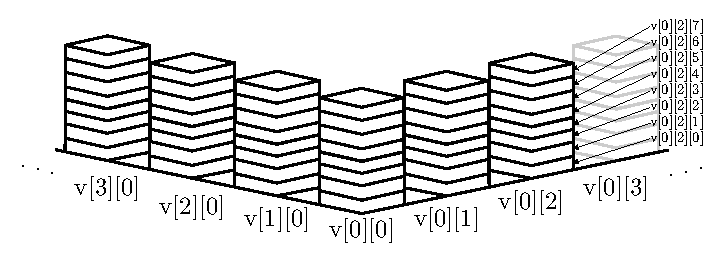
\includegraphics[width=\textwidth]{images/array_visualization}
    \end{center}



\pagebreak



\section{Matrix Operations (when Dimensions are `Nice')}
\subsection{Addition and Subtraction of Matrices}
Suppose we have to matrices that we want to add:
\[
A =
\begin{bmatrix}
    0.0 & 1.0 & 2.0 & 3.0 & 4.0 & 5.0 & 6.0 & 7.0 \\
    0.0 & 1.0 & 2.0 & 3.0 & 4.0 & 5.0 & 6.0 & 7.0 \\
    0.0 & 1.0 & 2.0 & 3.0 & 4.0 & 5.0 & 6.0 & 7.0 \\
    0.0 & 1.0 & 2.0 & 3.0 & 4.0 & 5.0 & 6.0 & 7.0 \\
    0.0 & 1.0 & 2.0 & 3.0 & 4.0 & 5.0 & 6.0 & 7.0 \\
    0.0 & 1.0 & 2.0 & 3.0 & 4.0 & 5.0 & 6.0 & 7.0 \\
    0.0 & 1.0 & 2.0 & 3.0 & 4.0 & 5.0 & 6.0 & 7.0 \\
    0.0 & 1.0 & 2.0 & 3.0 & 4.0 & 5.0 & 6.0 & 7.0
\end{bmatrix}, \quad
B =
\begin{bmatrix}
    0.0 & 1.0 & 2.0 & 3.0 & 4.0 & 5.0 & 6.0 & 7.0 \\
    0.0 & 1.0 & 2.0 & 3.0 & 4.0 & 5.0 & 6.0 & 7.0 \\
    0.0 & 1.0 & 2.0 & 3.0 & 4.0 & 5.0 & 6.0 & 7.0 \\
    0.0 & 1.0 & 2.0 & 3.0 & 4.0 & 5.0 & 6.0 & 7.0 \\
    0.0 & 1.0 & 2.0 & 3.0 & 4.0 & 5.0 & 6.0 & 7.0 \\
    0.0 & 1.0 & 2.0 & 3.0 & 4.0 & 5.0 & 6.0 & 7.0 \\
    0.0 & 1.0 & 2.0 & 3.0 & 4.0 & 5.0 & 6.0 & 7.0 \\
    0.0 & 1.0 & 2.0 & 3.0 & 4.0 & 5.0 & 6.0 & 7.0
\end{bmatrix}.
\]

\noindent We can quite easily implement this using intrinsics. Consider the following \texttt{C++} program.

\inputminted[tabsize=2,breaklines,linenos]{c++}{source/mat_add.cpp}

As expected, it outputs the sum, as shown below:
\[
C =
\begin{bmatrix}
    0.0 & 2.0 & 4.0 & 6.0 & 8.0 & 10.0 & 12.0 & 14.0 \\
    0.0 & 2.0 & 4.0 & 6.0 & 8.0 & 10.0 & 12.0 & 14.0 \\
    0.0 & 2.0 & 4.0 & 6.0 & 8.0 & 10.0 & 12.0 & 14.0 \\
    0.0 & 2.0 & 4.0 & 6.0 & 8.0 & 10.0 & 12.0 & 14.0 \\
    0.0 & 2.0 & 4.0 & 6.0 & 8.0 & 10.0 & 12.0 & 14.0 \\
    0.0 & 2.0 & 4.0 & 6.0 & 8.0 & 10.0 & 12.0 & 14.0 \\
    0.0 & 2.0 & 4.0 & 6.0 & 8.0 & 10.0 & 12.0 & 14.0 \\
    0.0 & 2.0 & 4.0 & 6.0 & 8.0 & 10.0 & 12.0 & 14.0
\end{bmatrix}.
\]

If we wanted to change this program so that it subtracts the matrices instead of add, one would change Line 40 to:
\mint{c++}|c[i][j] = _mm256_sub_ps(a[i][j], b[i][j]);|

\subsection{Multiplication of Matrices}
Suppose we have to matrices that we want to multiply:
\[
A =
\begin{bmatrix}
    0.0 & 1.0 & 2.0 & 3.0 & 4.0 & 5.0 & 6.0 & 7.0 \\
    0.0 & 1.0 & 2.0 & 3.0 & 4.0 & 5.0 & 6.0 & 7.0 \\
    0.0 & 1.0 & 2.0 & 3.0 & 4.0 & 5.0 & 6.0 & 7.0 \\
    0.0 & 1.0 & 2.0 & 3.0 & 4.0 & 5.0 & 6.0 & 7.0 \\
    0.0 & 1.0 & 2.0 & 3.0 & 4.0 & 5.0 & 6.0 & 7.0 \\
    0.0 & 1.0 & 2.0 & 3.0 & 4.0 & 5.0 & 6.0 & 7.0 \\
    0.0 & 1.0 & 2.0 & 3.0 & 4.0 & 5.0 & 6.0 & 7.0 \\
    0.0 & 1.0 & 2.0 & 3.0 & 4.0 & 5.0 & 6.0 & 7.0
\end{bmatrix}, \quad
B =
\begin{bmatrix}
    0.0 & 1.0 & 2.0 & 3.0 & 4.0 & 5.0 & 6.0 & 7.0 \\
    0.0 & 1.0 & 2.0 & 3.0 & 4.0 & 5.0 & 6.0 & 7.0 \\
    0.0 & 1.0 & 2.0 & 3.0 & 4.0 & 5.0 & 6.0 & 7.0 \\
    0.0 & 1.0 & 2.0 & 3.0 & 4.0 & 5.0 & 6.0 & 7.0 \\
    0.0 & 1.0 & 2.0 & 3.0 & 4.0 & 5.0 & 6.0 & 7.0 \\
    0.0 & 1.0 & 2.0 & 3.0 & 4.0 & 5.0 & 6.0 & 7.0 \\
    0.0 & 1.0 & 2.0 & 3.0 & 4.0 & 5.0 & 6.0 & 7.0 \\
    0.0 & 1.0 & 2.0 & 3.0 & 4.0 & 5.0 & 6.0 & 7.0
\end{bmatrix}.
\]

With slight modifications to our previous program, we can attempt to take the product.
\inputminted[tabsize=2,breaklines,linenos]{c++}{source/mat_mult.cpp}

This outputs the product:
\[
C =
\begin{bmatrix}
    0.0 & 1.0 & 4.0 & 9.0 & 16.0 & 25.0 & 36.0 & 49.0 \\
    0.0 & 1.0 & 4.0 & 9.0 & 16.0 & 25.0 & 36.0 & 49.0 \\
    0.0 & 1.0 & 4.0 & 9.0 & 16.0 & 25.0 & 36.0 & 49.0 \\
    0.0 & 1.0 & 4.0 & 9.0 & 16.0 & 25.0 & 36.0 & 49.0 \\
    0.0 & 1.0 & 4.0 & 9.0 & 16.0 & 25.0 & 36.0 & 49.0 \\
    0.0 & 1.0 & 4.0 & 9.0 & 16.0 & 25.0 & 36.0 & 49.0 \\
    0.0 & 1.0 & 4.0 & 9.0 & 16.0 & 25.0 & 36.0 & 49.0 \\
    0.0 & 1.0 & 4.0 & 9.0 & 16.0 & 25.0 & 36.0 & 49.0
\end{bmatrix}.
\]

However, this isn't correct! The product should be:

\[
C =
\begin{bmatrix}
    0.0 & 28.0 & 56.0 & 84.0 & 112.0 & 140.0 & 168.0 & 196.0 \\
    0.0 & 28.0 & 56.0 & 84.0 & 112.0 & 140.0 & 168.0 & 196.0 \\
    0.0 & 28.0 & 56.0 & 84.0 & 112.0 & 140.0 & 168.0 & 196.0 \\
    0.0 & 28.0 & 56.0 & 84.0 & 112.0 & 140.0 & 168.0 & 196.0 \\
    0.0 & 28.0 & 56.0 & 84.0 & 112.0 & 140.0 & 168.0 & 196.0 \\
    0.0 & 28.0 & 56.0 & 84.0 & 112.0 & 140.0 & 168.0 & 196.0 \\
    0.0 & 28.0 & 56.0 & 84.0 & 112.0 & 140.0 & 168.0 & 196.0 \\
    0.0 & 28.0 & 56.0 & 84.0 & 112.0 & 140.0 & 168.0 & 196.0
\end{bmatrix}.
\]

There are two choices for trying to multiply these matrices:
\begin{enumerate}
  \item Change the algorithm so that we no longer use the intrinsic.
  \item Change the first matrix to $B^\text{T}$ so that we can still make use of the \texttt{\_mm256\_mul\_ps} intrinsic function.
\end{enumerate}
Both of these options have a performance penalty: either dropping the use of intrinsic functions, or taking a hit and transposing $B$. Since the purpose of this discussion is to use intrinsics, we will take the second option.

Below is the fixed (really stupid and hacky, which works only for this single example and not all arrays in general) code, which prints the correct output that was given above:
\inputminted[tabsize=2,breaklines,linenos]{c++}{source/mat_mult_fixed.cpp}

\setcounter{MaxMatrixCols}{16}

\[
\begin{bmatrix}
    v_{000} & \cdots & v_{007}\ \ \ \vline & \cdots & \vline & v_{0m0} & \cdots & v_{0m7} \\

    & \vdots & & \vdots & & & \vdots & \\

    v_{n00} & \cdots & v_{n07}\ \ \ \vline & \cdots & \vline & v_{nm0} & \cdots & v_{nm7} \\
\end{bmatrix}^T
\]

\[
\begin{bmatrix}
    v_{000} & \cdots & v_{700}\ \ \ \vline & \cdots & \vline & v_{(n-8)00} & \cdots & v_{n00} \\

    & \vdots & & \vdots & & & \vdots & \\

    v_{0m0} & \cdots & v_{0m7}\ \ \ \vline & \cdots & \vline & v_{nm0} & \cdots & v_{nm7} \\
\end{bmatrix}^T
\]

\subsection{What About When the Dimensions are not `Nice'?}
I'm working on it.



\pagebreak



\section{Jacobi Method: A Nontrivial Example}
Over the course of this section I explain how to implement a Jacobi Method solver using intrinsics.

\end{document}
